

\documentclass[bigger,aspectratio=169]{beamer}

\usepackage{style}
\usepackage{subfiles}


\title[STG vs GRIN] %optional
{Comparing STG and GRIN}

\author[P. Podlovics, Cs. Hruska, Andor Pénzes ] % (optional, for multiple authors)
{Péter Podlovics, Csaba Hruska, Andor Pénzes}

\institute[ELTE] % (optional)
{
	Eötvös Loránd University (ELTE), \\ Budapest, Hungary
}

\date{Haskell meetup} % (optional)



\begin{document}

{
	\usebackgroundtemplate{
\includegraphics[width=\paperwidth,height=\paperheight]{title.jpg}}%
	\frame{\vspace{2cm}\titlepage}
}

\begin{frame}
	\frametitle{Overview}
	\tableofcontents
\end{frame}

\begin{frame}[fragile]
\frametitle{Why functional?}

\begin{vfitemize}
	\item Declarativeness
	\begin{itemize}
		\item[pro:] can program on a higher abstraction level
	\end{itemize}
	\item Composability\\
	\begin{itemize}
		\item[pro:] can easily piece together smaller programs
		\item[con:] results in a lot of function calls
	\end{itemize}
	\item Functions are first class citizens
	\begin{itemize}
		\item[pro:] higher order functions
		\item[con:] unknown function calls
	\end{itemize}
\end{vfitemize}

\end{frame}

\begin{frame}[fragile]
\frametitle{High level overview}

\begin{minipage}{0.4\textwidth}
	\begin{center}
		Spineless Tagless G-machine
	\end{center}
	\begin{itemize}
		\item<2-> higher order functional language
		\item<3-> execution of lambda calculus
		\item<4-> implicit operational semantics
		% op.sem. is detached from the language
		% can't really guess how the program is executed just by looking at the code
		\item<5-> efficient code generation
	\end{itemize}
\end{minipage}
\hfill
\begin{minipage}{0.4\textwidth}
	\begin{center}
		Graph Reduction Intermediate Notation
	\end{center}
	\begin{itemize}
		\item<6-> first order imperative language
		\item<7-> unified back end for functional languages
		\item<8-> explicit operational semantics
		% op.sem. closely tied together with the language
		% all functional constructs can be expressed using really simple and transparent language constructs (transparent as in we see what is happening)
		\item<9-> aggressive code optimization 
	\end{itemize}
\end{minipage}

\end{frame}

%%%%%%%% STG Overview %%%%%%%%%%
\section{Spineless Tagless G-machine}

\begin{frame}[fragile]
\frametitle{STG overview}
\begin{center}

	\begin{minipage}{0.25\textwidth}
		\begin{figure}
			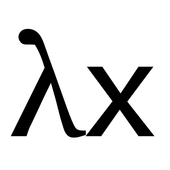
\includegraphics[scale=0.4]{lambda-icon.png}
		\end{figure}
	\end{minipage}
	\hfill
	\pause
	\begin{minipage}{0.30\textwidth}
		\begin{figure}
			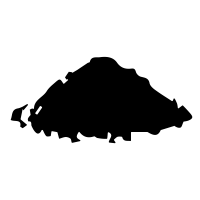
\includegraphics[scale=0.3]{heap-icon.png}
		\end{figure}
	\end{minipage}
	\hfill
	\pause
	\begin{minipage}{0.30\textwidth}
		\begin{figure}
			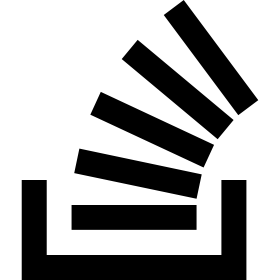
\includegraphics[scale=0.225]{stack-icon.png}
		\end{figure}
	\end{minipage}

\end{center}
\end{frame}

\begin{frame}[fragile]
\frametitle{STG overview}
\begin{center}

	\begin{minipage}{0.30\textwidth}
		\vspace{1cm}
		\begin{figure}
			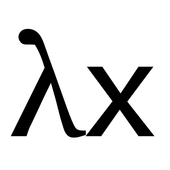
\includegraphics[scale=0.45]{lambda-icon.png}
		\end{figure}
		\onslide<2>
		\begin{haskellcode}
			and :: Bool -> Bool -> Bool
		\end{haskellcode}
		\vspace{-0.4cm}
		\onslide<2-3>
		\begin{haskellcode}
			and True True = True
			and _    _    = False
		\end{haskellcode}
	\end{minipage}
	\hfill
	\onslide<1-3>
	\begin{minipage}{0.30\textwidth}
		\begin{figure}
			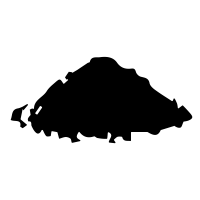
\includegraphics[scale=0.3]{heap-icon.png}
		\end{figure}
	\end{minipage}
	\hfill
	\begin{minipage}{0.30\textwidth}
		\begin{figure}
			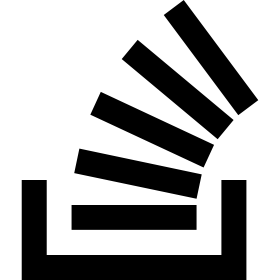
\includegraphics[scale=0.225]{stack-icon.png}
		\end{figure}
	\end{minipage}

\end{center}
\end{frame}

\begin{frame}[fragile]
\frametitle{STG overview}
\begin{center}

	\begin{minipage}{0.30\textwidth}
		\vspace{1.8cm}
		\begin{figure}
			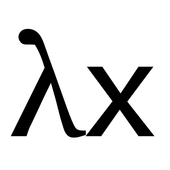
\includegraphics[scale=0.45]{lambda-icon.png}
		\end{figure}
		\begin{haskellcode}
			and x y = case x of
			  True -> case y of
			    True -> True
			    y' -> False
			  x' -> False
		\end{haskellcode}
	\end{minipage}
	\hfill
	\begin{minipage}{0.30\textwidth}
		\begin{figure}
			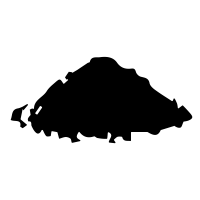
\includegraphics[scale=0.3]{heap-icon.png}
		\end{figure}
	\end{minipage}
	\hfill
	\begin{minipage}{0.30\textwidth}
		\begin{figure}
			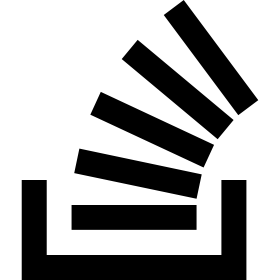
\includegraphics[scale=0.225]{stack-icon.png}
		\end{figure}
	\end{minipage}

\end{center}
\end{frame}

\begin{frame}[fragile]
\frametitle{STG overview}
\begin{center}

	\begin{minipage}{0.30\textwidth}
		\vspace{1.8cm}
		\begin{figure}
			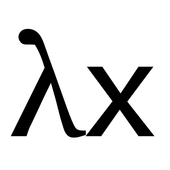
\includegraphics[scale=0.45]{lambda-icon.png}
		\end{figure}
		\begin{haskellcode}
			and = \x y -> case x of
			  True -> case y of
			    True -> True
			    y' -> False
			  x' -> False
		\end{haskellcode}
	\end{minipage}
	\hfill
	\begin{minipage}{0.30\textwidth}
		\begin{figure}
			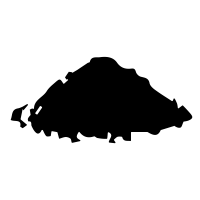
\includegraphics[scale=0.3]{heap-icon.png}
		\end{figure}
	\end{minipage}
	\hfill
	\begin{minipage}{0.30\textwidth}
		\begin{figure}
			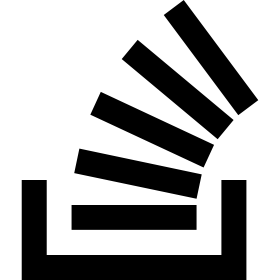
\includegraphics[scale=0.225]{stack-icon.png}
		\end{figure}
	\end{minipage}

\end{center}
\end{frame}

\begin{frame}[fragile]
\frametitle{STG overview}
\begin{center}

	\begin{minipage}{0.25\textwidth}
		\begin{figure}
			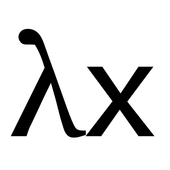
\includegraphics[scale=0.4]{lambda-icon.png}
		\end{figure}
	\end{minipage}
	\hfill
	\begin{minipage}{0.30\textwidth}
		\begin{figure}
			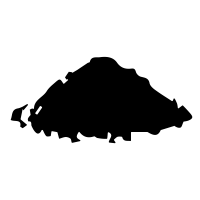
\includegraphics[scale=0.35]{heap-icon.png}
		\end{figure}
	\end{minipage}
	\hfill
	\begin{minipage}{0.30\textwidth}
		\begin{figure}
			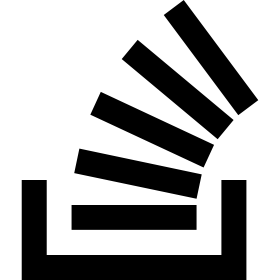
\includegraphics[scale=0.225]{stack-icon.png}
		\end{figure}
	\end{minipage}

\end{center}
\end{frame}

\begin{frame}[fragile]
\frametitle{STG overview}
\begin{center}

	\begin{minipage}{0.15\textwidth}
		\begin{figure}
			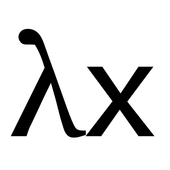
\includegraphics[scale=0.4]{lambda-icon.png}
		\end{figure}
	\end{minipage}
	\hfill
	\begin{minipage}{0.30\textwidth}
		\vspace{1cm}
		\begin{figure}
			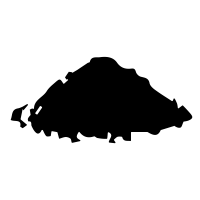
\includegraphics[scale=0.35]{heap-icon.png}
		\end{figure}
		\vspace{-1cm}
		\begin{figure}
			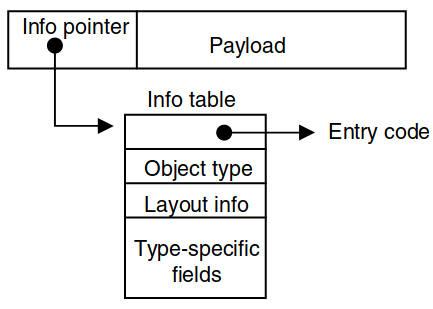
\includegraphics[scale=0.33]{heap-object.png}
		\end{figure}
	\end{minipage}
	\hfill
	\begin{minipage}{0.30\textwidth}
		\begin{figure}
			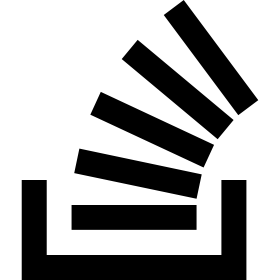
\includegraphics[scale=0.225]{stack-icon.png}
		\end{figure}
	\end{minipage}

\end{center}
\end{frame}

\begin{frame}[fragile]
\frametitle{STG overview}
\begin{center}

	\begin{minipage}{0.25\textwidth}
		\begin{figure}
			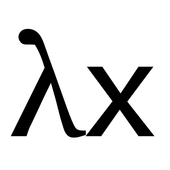
\includegraphics[scale=0.4]{lambda-icon.png}
		\end{figure}
	\end{minipage}
	\hfill
	\begin{minipage}{0.30\textwidth}
		\begin{figure}
			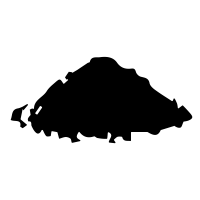
\includegraphics[scale=0.3]{heap-icon.png}
		\end{figure}
	\end{minipage}
	\hfill
	\begin{minipage}{0.30\textwidth}
		\begin{figure}
			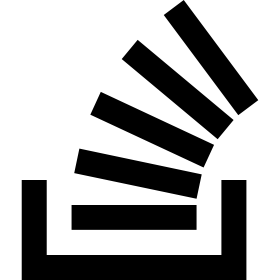
\includegraphics[scale=0.225]{stack-icon.png}
		\end{figure}
	\end{minipage}

\end{center}
\end{frame}

\begin{frame}[fragile]
\frametitle{STG overview}
\begin{center}

	\begin{minipage}{0.25\textwidth}
		\begin{figure}
			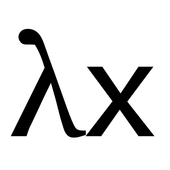
\includegraphics[scale=0.4]{lambda-icon.png}
		\end{figure}
	\end{minipage}
	\hfill
	\begin{minipage}{0.30\textwidth}
		\begin{figure}
			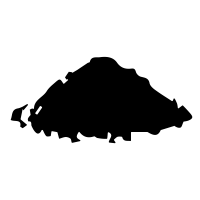
\includegraphics[scale=0.3]{heap-icon.png}
		\end{figure}
	\end{minipage}
	\hfill
	\begin{minipage}{0.30\textwidth}
		\vspace{1cm}
		\begin{figure}
			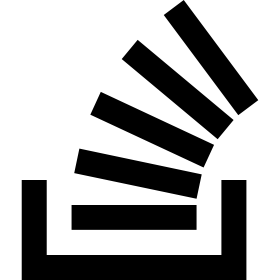
\includegraphics[scale=0.3]{stack-icon.png}
		\end{figure}
		\pause
		\begin{haskellcode}
			case * of {...}
		\end{haskellcode}
		\pause
		\begin{haskellcode}
			Update x *
		\end{haskellcode}
		\pause
		\begin{haskellcode}
			* x y z
		\end{haskellcode}
	\end{minipage}

\end{center}
\end{frame}

\begin{frame}[fragile]
\frametitle{STG overview}
\begin{center}

	\begin{minipage}{0.25\textwidth}
		\begin{figure}
			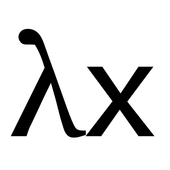
\includegraphics[scale=0.4]{lambda-icon.png}
		\end{figure}
	\end{minipage}
	\hfill
	\begin{minipage}{0.30\textwidth}
		\begin{figure}
			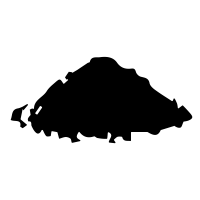
\includegraphics[scale=0.3]{heap-icon.png}
		\end{figure}
	\end{minipage}
	\hfill
	\begin{minipage}{0.30\textwidth}
		\begin{figure}
			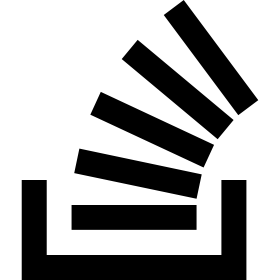
\includegraphics[scale=0.225]{stack-icon.png}
		\end{figure}
	\end{minipage}

\end{center}
\end{frame}

\begin{frame}[fragile]
\frametitle{STG overview}
\begin{center}

	\begin{minipage}{0.30\textwidth}
		\vspace{-3cm}
		\begin{haskellcode}
			and = \x y -> case x of
			 True -> case y of
			  True -> True
			   y' -> False
			 x' -> False
		\end{haskellcode}
	\end{minipage}
	\hfill
	\begin{minipage}{0.30\textwidth}
		\vspace{0.75cm}
		\begin{figure}
			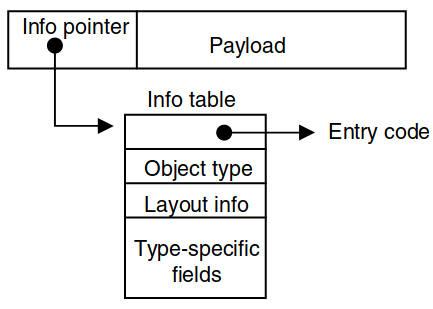
\includegraphics[scale=0.30]{heap-object.png}
		\end{figure}
	\end{minipage}
	\hfill
	\begin{minipage}{0.30\textwidth}
		\vspace{5cm}
		\begin{haskellcode}
			case * of {...}
			Update x *
			* x y z
		\end{haskellcode}
	\end{minipage}

\end{center}
\end{frame}

%%%%%%%%%% STG Examples %%%%%%%%%%%
\section{STG examples}

\begin{frame}[fragile]
\frametitle{STG id-add}
\begin{center}

	\begin{haskellcode}
		id = \x -> x
	\end{haskellcode}
	\pause
	\begin{haskellcode}
		zero = \ -> Int# 0#;
		one  = \ -> Int# 1#;
	\end{haskellcode}
	\pause
	\begin{haskellcode}
		add = \x y -> case x of
		  Int# x' -> case y of
		    Int# y' -> case +# x' y' of
		      r -> Int# r;
		    badInt -> Error_min badInt;
		  badInt -> Error_min badInt;
	\end{haskellcode}
	\pause
	\begin{haskellcode}
		main = \ -> let add_one = \ -> add one
		            in id add_one zero
	\end{haskellcode}

\end{center}
\end{frame}


\begin{frame}[fragile]
\frametitle{STG id-add}
\begin{center}

	\begin{haskellcode}
		id = \x -> x
	\end{haskellcode}
	\begin{haskellcode}
		zero = \ -> Int# 0#;
		one  = \ -> Int# 1#;
	\end{haskellcode}
	\begin{haskellcode}
		add = \x y -> case x of
		  Int# x' -> case y of
		    Int# y' -> case +# x' y' of
		      r -> Int# r;
		    badInt -> Error_min badInt;
		  badInt -> Error_min badInt;
	\end{haskellcode}
	\begin{haskellcode}
		main = \ => let add_one = \ -> add one
		            in id add_one zero
	\end{haskellcode}

\end{center}
\end{frame}

\section{STG demonstration}

\section{Graph Reduction Intermediate Notation}
%%%%%% GRIN Overview %%%%%%%%%

\begin{frame}[fragile]
\frametitle{GRIN overview}
\begin{center}

	\begin{minipage}{0.30\textwidth}
		\begin{figure}
			
\includegraphics[scale=0.20]{algebra.png}
		\end{figure}
	\end{minipage}
	\hfill
	\pause
	\begin{minipage}{0.30\textwidth}
		\begin{figure}
			
\includegraphics[scale=0.15]{graph-reduction.png}
		\end{figure}
	\end{minipage}
	\hfill
	\pause
	\begin{minipage}{0.30\textwidth}
		\begin{figure}
			
\includegraphics[scale=0.15]{whole-program-compilation.png}
		\end{figure}
	\end{minipage}

\end{center}
\end{frame}

\begin{frame}[fragile]
\frametitle{GRIN overview}
\begin{center}

	\begin{minipage}{0.30\textwidth}
		\begin{figure}
			
\includegraphics[scale=0.25]{algebra.png}
		\end{figure}
	\end{minipage}
	\hfill
	\begin{minipage}{0.30\textwidth}
		\begin{figure}
			
\includegraphics[scale=0.15]{graph-reduction.png}
		\end{figure}
	\end{minipage}
	\hfill
	\begin{minipage}{0.30\textwidth}
		\begin{figure}
			
\includegraphics[scale=0.15]{whole-program-compilation.png}
		\end{figure}
	\end{minipage}

\end{center}
\end{frame}

\begin{frame}[fragile]
\frametitle{GRIN overview}
\begin{center}

	\begin{minipage}{0.30\textwidth}
		\vspace{1cm}
		\begin{figure}
			
\includegraphics[scale=0.25]{algebra.png}
		\end{figure}
		\vspace{-0.5cm}
		\begin{itemize}
			\item<1-> C-node
			\item<2-> F-node
			\item<3-> P-node
		\end{itemize}
	\end{minipage}
	\hfill
	\begin{minipage}{0.30\textwidth}
		\begin{figure}
			
\includegraphics[scale=0.15]{graph-reduction.png}
		\end{figure}
	\end{minipage}
	\hfill
	\begin{minipage}{0.30\textwidth}
		\begin{figure}
			
\includegraphics[scale=0.15]{whole-program-compilation.png}
		\end{figure}
	\end{minipage}

\end{center}
\end{frame}


\begin{frame}[fragile]
\frametitle{GRIN overview}
\begin{center}

	\begin{minipage}{0.30\textwidth}
		\begin{figure}
			
\includegraphics[scale=0.20]{algebra.png}
		\end{figure}
	\end{minipage}
	\hfill
	\begin{minipage}{0.30\textwidth}
		\begin{figure}
			
\includegraphics[scale=0.20]{graph-reduction.png}
		\end{figure}
	\end{minipage}
	\hfill
	\begin{minipage}{0.30\textwidth}
		\begin{figure}
			
\includegraphics[scale=0.15]{whole-program-compilation.png}
		\end{figure}
	\end{minipage}

\end{center}
\end{frame}

\begin{frame}[fragile]
\frametitle{GRIN overview}
\begin{center}

	\begin{minipage}{0.30\textwidth}
		\begin{figure}
			
\includegraphics[scale=0.20]{algebra.png}
		\end{figure}
	\end{minipage}
	\hfill
	\begin{minipage}{0.30\textwidth}
		\vspace{1cm}
		\begin{figure}
			
\includegraphics[scale=0.20]{graph-reduction.png}
		\end{figure}
		\vspace{-0.5cm}
		\begin{itemize}
			\item<1-> store
			\item<2-> fetch
			\item<3-> update
		\end{itemize}
	\end{minipage}
	\hfill
	\begin{minipage}{0.30\textwidth}
		\begin{figure}
			
\includegraphics[scale=0.15]{whole-program-compilation.png}
		\end{figure}
	\end{minipage}

\end{center}
\end{frame}

\begin{frame}[fragile]
\frametitle{GRIN overview}
\begin{center}

	\begin{minipage}{0.30\textwidth}
		\begin{figure}
			
\includegraphics[scale=0.20]{algebra.png}
		\end{figure}
	\end{minipage}
	\hfill
	\begin{minipage}{0.30\textwidth}
		\begin{figure}
			
\includegraphics[scale=0.15]{graph-reduction.png}
		\end{figure}
	\end{minipage}
	\hfill
	\begin{minipage}{0.30\textwidth}
		\begin{figure}
			
\includegraphics[scale=0.20]{whole-program-compilation.png}
		\end{figure}
	\end{minipage}

\end{center}
\end{frame}

\begin{frame}[fragile]
\frametitle{GRIN overview}
\begin{center}

	\begin{minipage}{0.30\textwidth}
		\begin{figure}
			
\includegraphics[scale=0.20]{algebra.png}
		\end{figure}
	\end{minipage}
	\hfill
	\begin{minipage}{0.30\textwidth}
		\begin{figure}
			
\includegraphics[scale=0.15]{graph-reduction.png}
		\end{figure}
	\end{minipage}
	\hfill
	\begin{minipage}{0.30\textwidth}
		\vspace{1cm}
		\begin{figure}
			\includegraphics[scale=0.20]{whole-program-compilation.png}
		\end{figure}
		\vspace{-0.5cm}
		\begin{itemize}
			\item<1-> eval
			\item<2-> apply
			\item<3-> analyses
		\end{itemize}
	\end{minipage}

\end{center}
\end{frame}

\begin{frame}[fragile]
\frametitle{GRIN overview}
\begin{center}

	\begin{minipage}{0.30\textwidth}
		\vspace{1cm}
		\begin{figure}
			\includegraphics[scale=0.20]{algebra.png}
		\end{figure}
		\vspace{0.3cm}
		\begin{itemize}
			\item C-node
			\item F-node
			\item P-node
		\end{itemize}
	\end{minipage}
	\hfill
	\begin{minipage}{0.30\textwidth}
		\begin{figure}
			\includegraphics[scale=0.15]{graph-reduction.png}
		\end{figure}
		\begin{itemize}
			\item store
			\item fetch
			\item update
		\end{itemize}
	\end{minipage}
	\hfill
	\begin{minipage}{0.30\textwidth}
		\begin{figure}
			\includegraphics[scale=0.15]{whole-program-compilation.png}
		\end{figure}
		\begin{itemize}
			\item eval
			\item apply
			\item analyses
		\end{itemize}
	\end{minipage}

\end{center}
\end{frame}


%%%%%% GRIN Examples %%%%%%%%%
\section{GRIN examples}

\begin{frame}[fragile]
\frametitle{GRIN id}

\begin{center}

	\vspace{0.5cm}
	\begin{minipage}{0.40\textwidth}
		\begin{haskellcode}
			id x.0 =
			 x.0' <- eval x.0
			 pure x.0'
		\end{haskellcode}
		\vfill
		\pause
		\begin{haskellcode}
			eval p =
			 v <- fetch p
			 case v of
			  (CInt _n) -> pure v
			  (Fid x.1) ->
			   r.id <- id x.1
			   update p r.id
			   pure r.id
		\end{haskellcode}
	\end{minipage}
	\hfill
	\pause
	\begin{minipage}{0.50\textwidth}
		\begin{haskellcode}
			id_one =
			 one   <- pure (CInt 1)
			 ptr   <- store one
			 thunk <- pure (Fid ptr)
			 pure thunk
		\end{haskellcode}
		\vspace{1.55cm}
		\pause
		\begin{haskellcode}
			grinMain =
			 (CInt k) <- eval id_one
			 _prim_int_print k
		\end{haskellcode}
	\end{minipage}

\end{center}
\end{frame}

\begin{frame}[fragile]
\frametitle{GRIN add}

\begin{center}
	
	\vspace{0.4cm}
	\begin{minipage}{0.45\textwidth}
		\begin{haskellcode}
			add x y =
			 (CInt x') <- eval x
			 (CInt y') <- eval y
			 r <- _int_add x' y'
			 pure (CInt r)
		\end{haskellcode}
		\pause
		\begin{haskellcode}
			eval p =
			 v <- fetch p
			 case v of
			  (CInt _n) -> pure v
			  (Fadd x.1 y.1) ->
			   r.add <- add x.1 y.1
			   update p r.add
			   pure r.add
		\end{haskellcode}
	\end{minipage}
	\hfill
	\pause
	\begin{minipage}{0.50\textwidth}
		\begin{haskellcode}
			add_one =
			 one <- store (CInt 1)
			 pure (P1_add one)
		\end{haskellcode}
		\pause
		\begin{haskellcode}
			grinMain =
			 zero <- store (CInt 0)
			 suc <- add_one
			 apply suc zero
		\end{haskellcode}
		\vfill
		\pause
		\begin{haskellcode}
			apply f u =
			 case f of
			  (P2_add) ->
			   pure (P1_add u)
			  (P1_add z) -> add z u
		\end{haskellcode}
	\end{minipage}

\end{center}
\end{frame}

\begin{frame}[fragile]
\frametitle{GRIN add}
\begin{center}

	\vspace{0.4cm}
	\begin{minipage}{0.45\textwidth}
		\begin{haskellcode}
			add x y =
			 <...>
		\end{haskellcode}
		\begin{haskellcode}
			eval p =
			 v <- fetch p
			 case v of
			  (CInt _n) -> pure v
			  (P2_add) -> pure v
			  (P1_add _x) -> pure v
			  (Fadd x.1 y.1) ->
			   r.add <- add x.1 y.1
			   update p r.add
			   pure r.add
		\end{haskellcode}
	\end{minipage}
	\hfill
	\begin{minipage}{0.50\textwidth}
		\begin{haskellcode}
			add_one =
			 one <- store (CInt 1)
			 pure (P1_add one)
		\end{haskellcode}
		\vfill
		\begin{haskellcode}
			grinMain =
			 zero <- store (CInt 0)
			 suc <- add_one
			 apply suc zero
		\end{haskellcode}
		\vfill
		\begin{haskellcode}
			apply f u =
			 case f of
			  (P2_add) ->
			   pure (P1_add u)
			  (P1_add z) -> add z u
		\end{haskellcode}
	\end{minipage}

\end{center}
\end{frame}


\begin{frame}[fragile]
\frametitle{GRIN id-add}
\begin{center}

	\begin{minipage}{0.40\textwidth}
		\begin{haskellcode}
			id q =
			 q' <- eval q
			 pure q'
		\end{haskellcode}
		\begin{haskellcode}
			add x y =
			 (CInt x') <- eval x
			 (CInt y') <- eval y
			 r <- _int_add x' y'
			 pure (CInt r)
		\end{haskellcode}
		\begin{haskellcode}
			eval p = ...
		\end{haskellcode}
		\begin{haskellcode}
			apply f u = ...
		\end{haskellcode}
	\end{minipage}
	\hfill
	%TODO: step-by-step for grinMain
	\begin{minipage}{0.55\textwidth}
		\begin{haskellcode}
			-- id (add 1) 0 ?
		\end{haskellcode}
		\vspace{-0.60cm}
		\pause
		\begin{haskellcode}
		grinMain =
		 zero <- store (CInt 0)
		 one  <- store (CInt 1)

		 add_1 <- store (P1_add one)
		 thunk <- store (Fid add_1)

		 id_add_1 <- eval thunk
		 r <- apply id_add_1 zero

		 (CInt r) <- pure r
		 _prim_int_print r
		\end{haskellcode}
	\end{minipage}

\end{center}
\end{frame}

\section{GRIN demonstration}

\begin{frame}
\frametitle{Consequences of the execution models}

\begin{minipage}{0.45\textwidth}
	\vspace{0.3cm}
	\begin{center}
		STG
	\end{center}
	\begin{itemize}
		\item<1-> closures:
		\begin{itemize}
			\item<2-> represented by heap objects
			\item<3-> they need special treatment
			\item<4-> generic data layout
			\item<5-> not representable in a register
		\end{itemize}
		\item<6-> execution stack:
		\begin{itemize}
			\item<7-> custom stack
			\item<8-> custom calling convention for LLVM
		\end{itemize}
	\end{itemize}
\end{minipage}
\hfill
\begin{minipage}{0.45\textwidth}
	\begin{center}
		GRIN
	\end{center}
	\begin{itemize}
		\item<9-> closures:
		\begin{itemize}[leftmargin=-2cm]
			\item<10-> only data, no builtins
			\item<11-> standard optimizations work
			\item<12-> custom data layout \\(C-style tagged union)
			\item<13-> can be put into registers
		\end{itemize}
		\item<14-> execution stack:
		\begin{itemize}
			\item<15-> standard C execution model
			\item<16-> we get LLVM for free
		\end{itemize}
	\end{itemize}
\end{minipage}

\end{frame}

{ %TODO: FIX
	\usebackgroundtemplate{\includegraphics[width=\paperwidth,height=\paperheight]{title.jpg}}%
	\begin{frame}{}
	
	\vspace{2cm}
	
	{\bf\Huge\color{white} THANK YOU}
	
	\bigskip
	
	{\bf\Huge\color{white} FOR YOUR}
	
	\bigskip
	
	{\bf\Huge\color{white} ATTENTION!}
	
 \end{frame}
}

\end{document}





